\newcommand\WIDTH{3cm}
\newcommand\HEIGHT{1.25cm}
\newcommand\Ydist{0.2cm}
\newcommand\XPOS{1cm}
\newcommand\TOTheight{6.2cm}
\newcommand\TOTwidth{4cm}
\newcommand\PTS{1.2pt}
\newcommand\SHADOWred{50}
\newcommand\SHADOWgreen{30}
\newcommand\SHADOWblue{20}

\newcommand\blockHeight{1.5cm}
\newcommand\blockWidth{4cm}

\centering

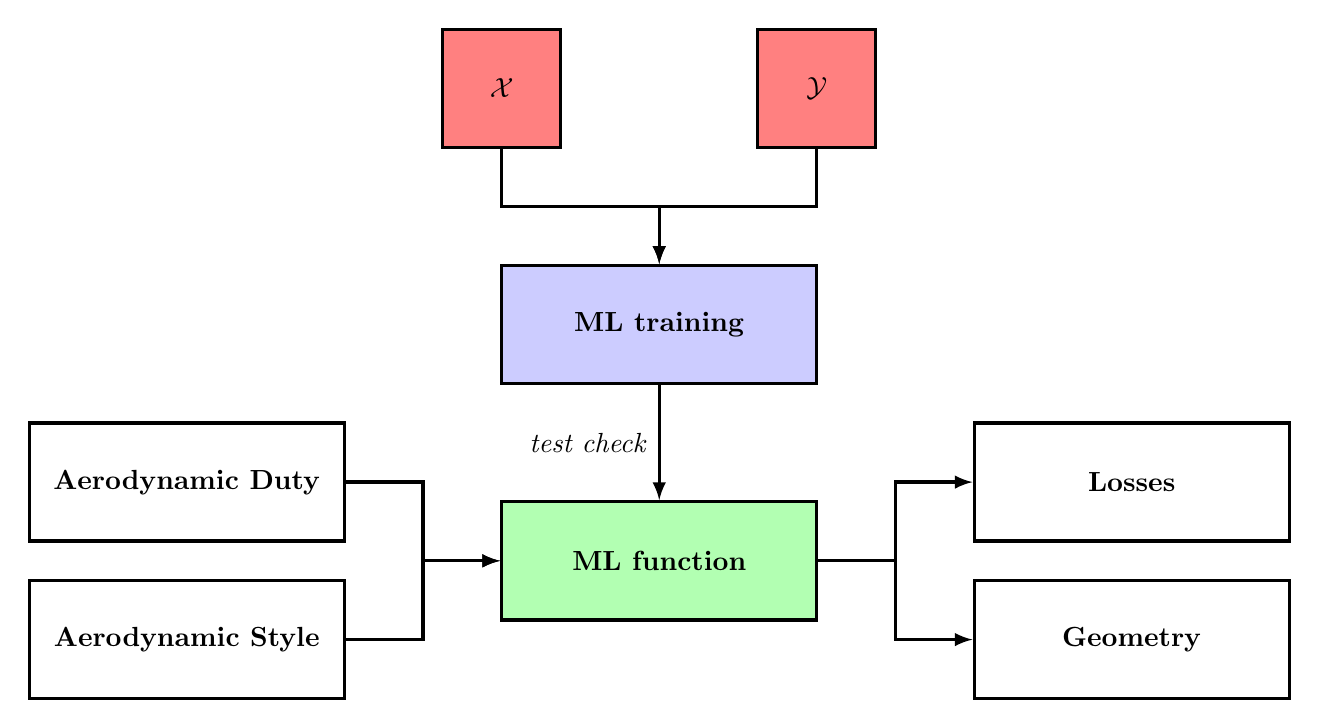
\begin{tikzpicture}
    
    \node[draw,
        rectangle,
        % rounded corners,
        line width = \PTS,
        minimum height = \blockHeight,
        minimum width = \blockWidth,
        fill = blue!\SHADOWblue,
    ] (AI) at (0, 0) {\textbf{ML training}};

    \node[draw,
        rectangle,
        % rounded corners,
        line width = \PTS,
        minimum height = \blockHeight,
        minimum width = \blockHeight,
        fill = red!\SHADOWred,
    ] (X) at (-2, 3) {$\mathcal{X}$};

    \node[draw,
        rectangle,
        % rounded corners,
        line width = \PTS,
        minimum height = \blockHeight,
        minimum width = \blockHeight,
        fill = red!\SHADOWred,
    ] (Y) at (2, 3) {$\mathcal{Y}$};

    \node[draw,
        rectangle,
        % rounded corners,
        line width = \PTS,
        minimum height = \blockHeight,
        minimum width = \blockWidth,
        fill = green!\SHADOWgreen,
    ] (func) at (0, -3) {\textbf{ML function}};
    
    \node[draw,
        rectangle,
        % rounded corners,
        line width = \PTS,
        minimum height = \blockHeight,
        minimum width = \blockWidth
    ] (inputDuty) at (-6, -2) {\textbf{Aerodynamic Duty}};

    \node[draw,
        rectangle,
        % rounded corners,
        line width = \PTS,
        minimum height = \blockHeight,
        minimum width = \blockWidth
    ] (inputStyle) at (-6, -4) {\textbf{Aerodynamic Style}};

    \node[draw,
        rectangle,
        % rounded corners,
        line width = \PTS,
        minimum height = \blockHeight,
        minimum width = \blockWidth
    ] (outputGeometry) at (6, -4) {\textbf{Geometry}};

    \node[draw,
        rectangle,
        % rounded corners,
        line width = \PTS,
        minimum height = \blockHeight,
        minimum width = \blockWidth
    ] (outputProperty) at (6, -2) {\textbf{Losses}};

    \coordinate[] (c1) at (-2, 1.5) {};
    \coordinate[] (c2) at (2,  1.5) {};
    \coordinate[] (c3) at (0,  1.5) {};
    \coordinate[] (c4) at (-3,  -2) {};
    \coordinate[] (c5) at (-3,  -4) {};
    \coordinate[] (c6) at (-3,  -3) {};
    \coordinate[] (c7) at (3,  -2) {};
    \coordinate[] (c8) at (3,  -4) {};
    \coordinate[] (c9) at (3,  -3) {};

    \draw[-latex, line width=\PTS] (X.south) -- (c1) -- (c3) to (AI.north);
    \draw[-latex, line width=\PTS] (Y.south) -- (c2) -- (c3) to (AI.north);
    \draw[-latex, line width=\PTS] (AI) -- node[anchor=east] {\textit{test check}} (func);
    \draw[-latex, line width=\PTS] (inputDuty.east)  -- (c4) -- (c6) to (func.west);
    \draw[-latex, line width=\PTS] (inputStyle.east) -- (c5) -- (c6) to (func.west);
    \draw[-latex, line width=\PTS] (func.east) -- (c9) -- (c7) to (outputProperty.west);
    \draw[-latex, line width=\PTS] (func.east) -- (c9) -- (c8) to (outputGeometry.west);

\end{tikzpicture}
